% !TEX root = main.tex

\section{频率域滤波} % Chap 4
\subsection{傅里叶级数与傅里叶变换}
\begin{definition}[傅里叶级数]
设$f(t)$为以$T$为周期的函数,绝对可积,则$f(t)$可表示为
\[f(t)=\sum_{n=-\infty}^{\infty}c_n\ee^{j\frac{2\pi n}{T}t}\]
其中$j$为虚数单位,
\[c_n=\frac{1}{T}\intabu{-T/2}{T/2}{f(t)\ee^{-j\frac{2\pi n}{T}t}}{t},\,n=0,\pm 1,\pm 2,\ldots\]
\end{definition}

傅里叶级数中每一个基函数都是一个单频谐波,对应的系数/频谱表明原函数对这种频率成分贡献的大小(原函数在这个谐波上的投影)

\begin{definition}[冲激/狄利克$\delta$函数]
面积为1的长方形不断压扁,最后变成宽为0,高为无穷大的函数(左侧为连续情况,右侧为离散情况)
\[\delta(t)=\begin{cases}
\infty & t=0\\
0 & t\ne 0
\end{cases}\qquad
\delta(x)=\begin{cases}
1 & x=0\\
0 & x\ne 0
\end{cases}\]
即
\[\intab{-\infty}{\infty}{\delta(t)}=1
\qquad
\sum_{x=-\infty}^{\infty}\delta(x)=1\]
具有取样(sifting)特性
\[\intab{-\infty}{\infty}{f(t)\delta(t-t_0)}=f(t_0)
\qquad
\sum_{x=-\infty}^{\infty}f(x)\delta(x-x_0)=f(x_0)\]
\end{definition}
\begin{definition}[冲激串]
无限多个分离的周期冲激单元$\Delta T$之和
\[s_{\Delta T}(t)=\sum_{n=-\infty}^{\infty}\delta(t-n\Delta T)\]
\end{definition}
\begin{figure}[H]
\centering
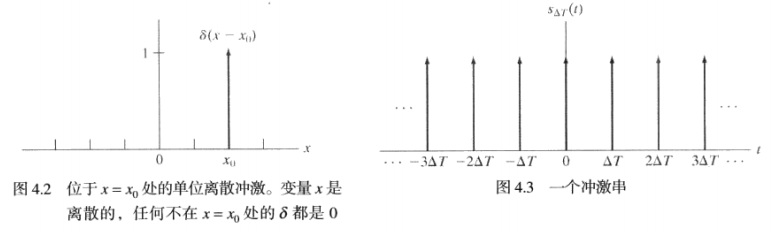
\includegraphics[width=0.8\linewidth]{fig/impulse.png}
\end{figure}

\begin{definition}[傅里叶变换与反变换]
连续情形的傅里叶变换(函数投影,取负号得共轭)和反变换为
\[\begin{aligned}
F(u)&=\Im[f(t)]=\intabu{-\infty}{+\infty}{f(t)\ee^{-j 2\pi ut}}{t}\\
f(t)&=\Im^{-1}[F(u)]=\intabu{-\infty}{+\infty}{F(u)\ee^{j 2\pi ut}}{u}
\end{aligned}\]
这两者构成一个傅里叶变换对。
对于离散情形有
\[\begin{aligned}
F(u)&=\sum_{x=0}^{M-1}f(x)\ee^{-j2\pi ux/M}\\
f(x)&=\frac{1}{M}\sum_{u=0}^{M-1}F(u)\ee^{j2\pi ux/M}
\end{aligned}\]
\end{definition}
由于傅里叶变换是$f(t)$乘上正弦项的展开,正弦项的频率由$\mu$决定(变量$t$已经被积分),积分后只剩下频率,故称傅里叶变换域是频率域。
注意坐标轴已经变化了,现在\textbf{横轴为频率}。

\begin{example}
矩形函数
\[f(t)=\begin{cases}
A & -W/2\leq t\leq W/2\\
0 & \text{otherwise}
\end{cases}\]
的傅里叶变换为
\[\begin{aligned}
F(u)&=\intabu{-W/2}{W/2}{A\ee^{-j2\pi ut}}{t}\\
&=\frac{-A}{j2\pi\mu}[\ee^{-j2\pi\mu W}-\ee^{j2\pi\mu W}]\\
&=AW\frac{\sin(\pi\mu W)}{\pi\mu W}=AW\sinc(\mu W)
\end{aligned}\]
\end{example}
\begin{example}
冲激的傅里叶变换(由取样特性)
\[F(\mu)=\intabu{-\infty}{\infty}{\delta(t)\ee^{-j2\pi\mu t}}{t}=\ee^{-j2\pi\mu 0}=1\]
而位于$t=t_0$的冲激傅里叶变换为
\[F(\mu)=\intabu{-\infty}{\infty}{\delta(t-t_0)\ee^{-j2\pi\mu t}}{t}=\ee^{-j2\pi\mu t_0}\]
周期冲激串的傅里叶变换
\[S(\mu)=\Im[s_{\Delta T}(t)]=\frac{1}{\Delta T}\sum_{n=-\infty}^{\infty}\delta\lrp{\mu-\frac{n}{\Delta T}}\]
\end{example}

\begin{definition}[卷积]
连续情形有
\[f(t)*h(t)=\intabu{-\infty}{+\infty}{f(\tau)h(t-\tau)}{\tau}\]
离散情形有
\[f(x)*h(x)=\sum_{m=0}^{M-1}f(m)h(x-m)\]
\end{definition}
\begin{theorem}[卷积定理]
建立起空间域和频率域\footnote{$t$所在的域称为空间域,$\mu$所在的域称为频率域}的联系
\[f(t)*h(t)\iff F(\mu)H(\mu)
\qquad
f(t)h(t)\iff F(\mu)*H(\mu)\]
即空间域两个函数卷积的傅里叶变换等于两个函数的傅里叶变换在频率域的乘积
\end{theorem}
\begin{analysis}
\[\begin{aligned}
\Im[f(t)*h(t)]&=\intabu{-\infty}{\infty}{\lrs{\intabu{-\infty}{\infty}{f(\tau)h(t-\tau)}{\tau}}\ee^{-j2\pi\mu t}}{t}\\
&=\intabu{-\infty}{\infty}{f(\tau)\lrs{\intabu{-\infty}{\infty}{h(t-\tau)\ee^{-j2\pi\mu t}}{t}}}{\tau}\\
&=\intabu{-\infty}{\infty}{f(\tau)\lrs{H(\mu)\ee^{-j2\pi\mu\tau}}}{\tau}\\
&=H(\mu)\intabu{-\infty}{\infty}{f(\tau)\lrs{\ee^{-j2\pi\mu\tau}}}{\tau}\\
&=H(\mu)F(\mu)
\end{aligned}\]
\end{analysis}

\subsection{取样函数}
\begin{example}
求取样函数
\[\tilde{f}(t)=f(t)s_{\Delta T}(t)=\sum_{n=-\infty}^{\infty}f(t)\delta(t-n\Delta T)\]
的傅里叶变换
\end{example}
\begin{analysis}
由卷积定理
\[\begin{aligned}
\tilde{F}(u)&=\Im[\tilde{f}(t)]=\Im[f(t)s_{\Delta T}(t)]\\
&=F(u)*S(u)=\intabu{-\infty}{\infty}{F(\tau)S(u-\tau)}{\tau}\\
&=\frac{1}{\Delta T}\intabu{-\infty}{\infty}{F(\tau)\sum_{n=-\infty}^{\infty}\delta\lrp{u-\tau-\frac{n}{\Delta T}}}{\tau}\\
&=\frac{1}{\Delta T}\sum_{n=-\infty}^{\infty}F\lrp{u-\frac{n}{\Delta T}}
\end{aligned}\]
\end{analysis}

\begin{theorem}[奈奎斯特(Nyquist)采样定理]
如果以超过函数最高频率的两倍的采样率来获得样本,则连续的带限函数\footnote{对于以原点为中心的有限区间(带宽)之外的频率值,其傅里叶变换为零。
}可以完全从它的样本集恢复,即
\[\frac{1}{\Delta T}>2\mu_{\max}\]
\end{theorem}

若以低于两倍的采样率来采样则会出现混淆现象
\begin{figure}[H]
\centering
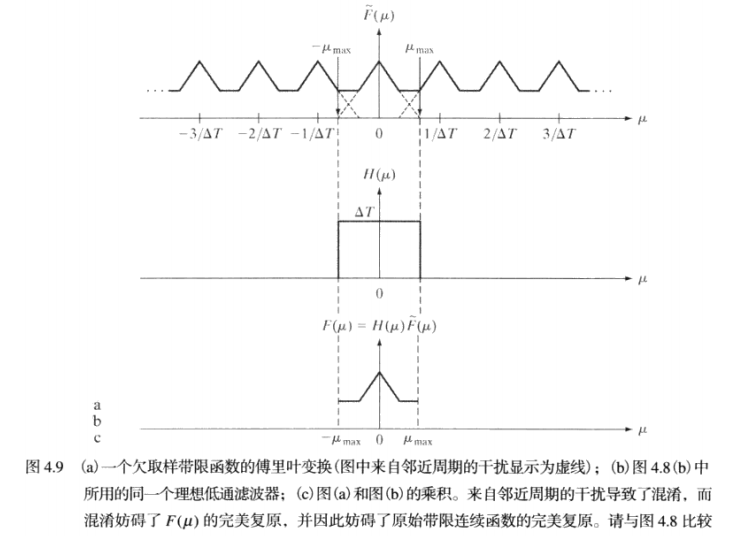
\includegraphics[width=0.8\linewidth]{fig/nyquist.png}
\end{figure}

由取样数据重建函数
\[f(t)=\sum_{n=-\infty}^{\infty}f(n\Delta T)\sinc\lrs{\frac{t-n\Delta T}{\Delta T}}\]

\subsection{二维傅里叶变换}
\begin{definition}[二维冲激]
\[\delta(t,z)=\begin{cases}
\infty & t=z=0\\
0 & \text{otherwise}
\end{cases}\qquad
\delta(x,y)=\begin{cases}
1 & x=y=0\\
0 & \text{otherwise}
\end{cases}\]
有取样特性
\[\sum_{x=-\infty}^\infty\sum_{y=-\infty}^\infty f(x,y)\delta(x-x_0,y-y_0)=f(x_0,y_0)\]
\end{definition}
\begin{definition}[二维离散傅里叶变换]
二维连续傅里叶变换对
\[\begin{aligned}
F(u,v)&=\intabu{-\infty}{\infty}{\intabu{-\infty}{\infty}{f(t,z)\ee^{-j2\pi(ut+vz)}}{t}}{z}\\
f(t,z)&=\intabu{-\infty}{\infty}{\intabu{-\infty}{\infty}{F(u,v)\ee^{j2\pi(ut+vz)}}{u}}{v}
\end{aligned}\]
二维离散傅里叶变换对
\[\begin{aligned}
F(u,v)&=\sum_{x=0}^{M-1}\sum_{y=0}^{N-1}f(x,y)\ee^{-2j\pi (ux/M+vy/N)}\\
f(x,y)&=\frac{1}{MN}\sum_{u=0}^{M-1}\sum_{v=0}^{N-1}F(u,v)\ee^{2\pi j(ux/M+vy/N)}
\end{aligned}\]
\end{definition}
\begin{theorem}[二维采样定理]
二维取样基于二维冲激串
\[\tilde{f}(t,z)=f(t,z)s_{\Delta T\Delta Z}(t,z)=\sum_{m=-\infty}^{\infty}\sum_{n=-\infty}^{\infty}f(t,z)\delta(t-m\Delta T,z-n\Delta Z)\]
取样率需要满足
\[\frac{1}{\Delta T}>2\mu_{\max}\qquad\frac{1}{\Delta Z}>2v_{\max}\]
\end{theorem}
\begin{definition}[傅里叶谱和相角]
由于二维DFT通常为复函数,因此用极坐标形式表示
\[F(u,v)=|F(u,v)|\ee^{j\varphi(u,v)}\]
其中幅度
\[|F(u,v)|=\sqrt{\Real^2(u,v)+\Imag^2(u,v)}\]
称为傅里叶谱,而
\[\varphi(u,v)=\arctan\lrs{\frac{\Imag(u,v)}{\Real(u,v)}}\]
为相角,
\[P(u,v)=|F(u,v)|^2\]
为功率谱
\end{definition}

注意$F(u,v)$的大小只是代表某一频率分量的数目,类似于直方图的概念。
频率域的坐标轴为$u,v$,因此中心点为$(0,0)$,
\[F(0,0)=\sum_{x=0}^{M-1}\sum_{y=0}^{N-1}f(x,y)=MN\bar{f}(x,y)\]
为图像的平均灰度。
即$u$方向和$v$方向上最低频的位置,零点处两个方向的频率都为零,因此这个量经常也被称为频谱的直流分量(DC)。

\begin{example}[陷波滤波器(notch filter)]
使得处理后的图像均值为0,从而使图像的整体灰度降低
\[H(u,v)=\begin{cases}
0 & (u,v)=(M/2,N/2)\\
1 & \text{others}
\end{cases}\]
\end{example}

\begin{figure}[H]
\centering
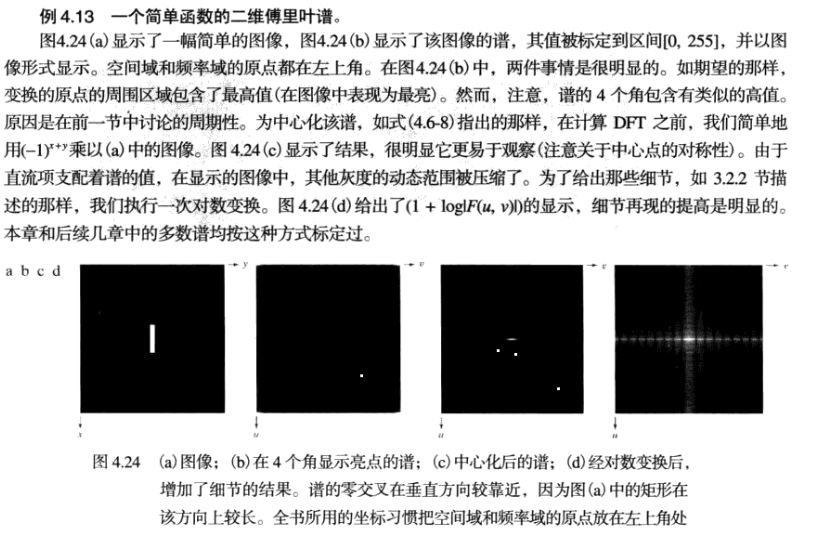
\includegraphics[width=\linewidth]{fig/fourier_spectrum.png}
\end{figure}

\textbf{相角对形状起着决定性作用!灰度信息则由谱携带。}
\begin{figure}[H]
\centering
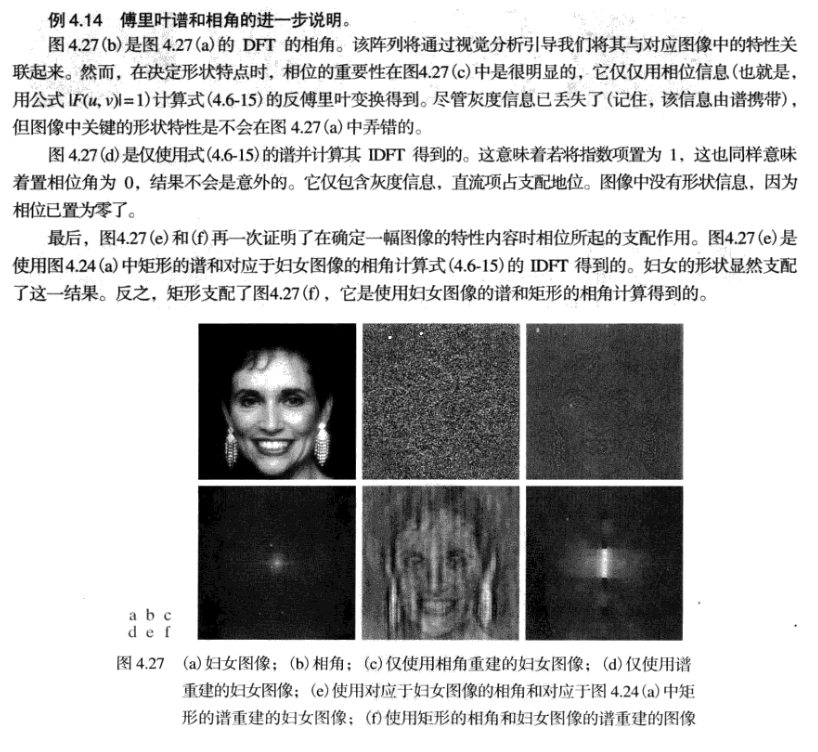
\includegraphics[width=\linewidth]{fig/spectrum_angle_example.png}
\end{figure}

\begin{theorem}[二维卷积定理]
二维的卷积定义如下
\[f(x,y)*h(x,y)=\sum_{m=0}^{M-1}\sum_{n=0}^{N-1}f(m,n)h(x-m,y-n)\]
同样有傅里叶变换对
\[\begin{aligned}
f(x,y)*h(x,y)\iff F(u,v)H(u,v)\\
f(x,y)h(x,y) \iff F(u,v)*H(u,v)
\end{aligned}\]
\end{theorem}
注意周期靠近会导致互相干扰而导致缠绕错误,因此需要进行零延拓(padding)。

假设函数$f(x)$和$h(x)$分别有$A$个和$B$个点组成,对这两个函数同时添加零,使其具有相同的周期
\[f_e=\begin{cases}
f(x) & 0\leq A-1\\
0 & A\leq x\leq P
\end{cases}
\qquad
h_e=\begin{cases}
h(x) & 0\leq x\leq B-1\\
0 & B\leq x\leq P
\end{cases}\]
同样对于二维图像滤波,若$f(x,y)$大小为$A\times B$,$h(x,y)$大小为$C\times D$,则延拓函数
\[f_e(x,y)=\begin{cases}
f(x,y) & 0\leq x\leq A-1\land 0\leq y\leq B-1\\
0 & A\leq x\leq P\lor B\leq y\leq Q
\end{cases}
\qquad
h_e(x,y)=\begin{cases}
h(x,y) & 0\leq x\leq C-1\land 0\leq y\leq D-1\\
0 & C\leq x\leq P\lor D\leq y\leq Q
\end{cases}\]
其中$P\geq A+C-1$,$Q\geq B+D-1$,通常可取$P=2M$,$Q=2N$。

\begin{definition}[相关]
相关性相当于算内积
\[g(x,y)=f(x,y)\circ h(x,y)=\sum_{m=0}^{M-1}\sum_{n=0}^{N-1}f^\star(m,n)h(x+m,y+n)\]
\end{definition}
\begin{theorem}[相关定理]
\[\begin{aligned}
f(x,y)\circ h(x,y)&\iff F^\star(u,v)H(u,v)\\
f^\star(x,y)h(x,y)&\iff F(u,v)\circ H(u,v)
\end{aligned}\]
\end{theorem}


\subsection{频率域滤波}
之所以要到频率域做滤波,是因为直观且计算比空间滤波容易(卷积耗时)
\begin{itemize}
\item 低通滤波器:平滑/模糊图像,设$D(u,v)$为频率域中点$(u,v)$与频率矩形中心的距离,$D_0$为截止频率
\begin{center}
\begin{tabular}{c|c|c}\hline
理想(ILPF) & $n$阶布特沃斯(BLPF) & 高斯\\\hline
$H(u,v)=\begin{cases}1 & D(u,v)\leq D_0\\0 & D(u,v)>D_0\end{cases}$ &
$H(u,v)=\dfrac{1}{1+[D(u,v)/D_0]^{2n}}$ &
$H(u,v)=\ee^{-D^2(u,v)/2D_0^2}$\\\hline
\end{tabular}
\end{center}
原点在频率中心,半径为$r$的圆包含的功率为
\[\alpha=\lrp{\sum_u\sum_v \frac{P(u,v)}{P_T}}\times 100\%=\lrp{\sum_u\sum_v \frac{P(u,v)}{\sum_{u=0}^{M-1}\sum_{v=0}^{N-1}|F(u,v)|^2}}\times 100\%\]
由于截止频率点处跳变太直接,物理无法实现,故是理想滤波器;而且会产生滤波模糊和振铃现象。
一阶BLPF没有振铃,二阶BLPF振铃很小,随着阶数增高振铃增大,故通常用二阶。
\item 高通滤波器:$H_{hp}(u,v)=1-H_{lp}(u,v)$,锐化图像(噪声、边缘、细节),只获得高频特征,没有背景,留下细节
\begin{center}
\begin{tabular}{c|c|c}\hline
理想(IGPF) & $n$阶布特沃斯(BGPF) & 高斯\\\hline
$H(u,v)=\begin{cases}0 & D(u,v)\leq D_0\\1 & D(u,v)>D_0\end{cases}$ &
$H(u,v)=\dfrac{1}{1+[D_0/D(u,v)]^{2n}}$ &
$H(u,v)=1-\ee^{-D^2(u,v)/2D_0^2}$\\\hline
\end{tabular}
\end{center}
\item 拉普拉斯滤波
\[H(u,v)=-4\pi^2\lrs{(u-P/2)^2+(v-Q/2)^2}=-4\pi^2D^2(u,v)\]
前面的系数可以去掉。拉普拉斯图像由下式给出
\[\nabla^2f(x,y)=\Im^{-1}[H(u,v)F(u,v)]\]
图像增强可以由下式实现
\[g(x,y)=f(x,y)+c\nabla^2 f(x,y)\]
\item 高频增强滤波:锐化/加强图像,高频增强,细节变得明显
\[\begin{aligned}
F_{lp}(u,v)&=H_{lp}(u,v)F(u,v)\\
F_{hp}(u,v)&=F(u,v)-F_{lp}(u,v)\\
&=(1-H_{lp}(u,v))F(u,v)\\
&=H_{hp}(u,v)F(u,v)\\
G(u,v)&=F(u,v)+F_{hp}(u,v)\\
&=(1+H_{hp}(u,v))F(u,v)
\end{aligned}\]
其中$k=1$为钝化模板,$k>1$为高提升滤波
\item 同态滤波器:高频增强,整个图像亮度又不能太亮(一片的亮度与低频有关)$\implies$抑制低频/环境光,提升高频/细节
\[f(x,y)=i(x,y)r(x,y)\]
其中$i(x,y)\in(0,\infty)$为照射分量(影响低频,一片);$0<r(x,y)<1$,反射率影响边缘/高频。
先取对数,然后再做傅里叶变换,最后记得取指数返回
\[\ln f(x,y)=\ln i(x,y)+\ln r(x,y)\]
同态滤波器
\[H(u,v)=(r_H-r_L)[1-\ee^{-c(D^2(u,v)/D_0^2)}]+r_L\]
其中$c$用于控制滤波器函数斜面的锐化,$r_L<1$,$r_H>1$
\begin{figure}[H]
\centering
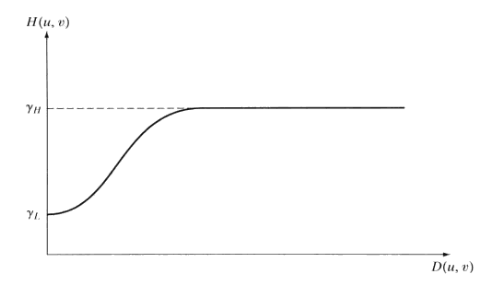
\includegraphics[width=0.4\linewidth]{fig/homo_filter.png}
\end{figure}
\end{itemize}

频率域滤波的步骤
\begin{figure}[H]
\centering
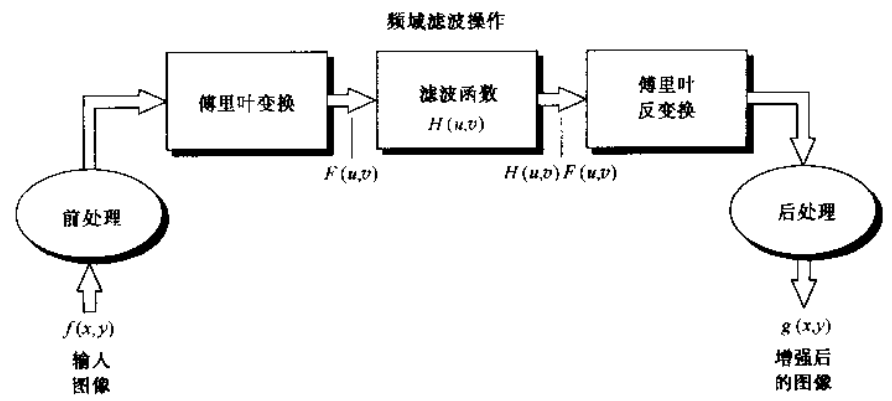
\includegraphics[width=0.6\linewidth]{fig/filter_pass.png}
\end{figure}
\begin{enumerate}
	\item 给定大小为$M\times N$的输入图像$f(x,y)$,选择填充参数$P=2M$,$Q=2N$
	\item 对$f(x,y)$添加必要的0,形成大小为$P\times Q$的填充后的图像$f_p(x,y)$
	\item 用$(-1)^{x+y}$乘以$f_p(x,y)$,做频谱中心化处理
	\item 用上面结果计算DFT,得到$F(u,v)$
	\item 生成一个\textbf{实对称}的滤波函数$H(u,v)$,大小为$P\times Q$,中心在$(P/2,Q/2)$处。
	用阵列相乘得到$G(u,v)=H(u,v)F(u,v)$
	\item 计算上式得到的IDFT,并恢复原图像
	\[g_p(x,y)=\Real[\Im[G(u,v)]](-1)^{x+y}\]
	\item 通过从$g_p(x,y)$的左上角提取$M\times N$大小的区域,得到最终结果$g(x,y)$
\end{enumerate}

\subsection{总结}
傅里叶变换的一些性质
\begin{itemize}
	\item 线性性:
	\[af_1(x,y)+bf_2(x,y)\iff aF_1(u,v)+bF_2(u,v)\]
	\item 平移性质:
	\[\begin{aligned}
	&f(x,y)\ee^{j2\pi(u_0x/M+v_0y/N)}\iff F(u-u_0,v-v_0)\\
	&f(x-x_0,y-y_0)\iff F(u,v)\ee^{-2j\pi(x_0u/M+y_0v/N)}
	\end{aligned}\]
	特别地,平移到频率矩形中心$(M/2,N/2)$
	\[\begin{aligned}
	&f(x,y)(-1)^{x+y}\iff F(u-M/2,v-N/2)\\
	&f(x-M/2,y-N/2)\iff F(u,v)(-1)^{u+v}
	\end{aligned}\]
	\item 旋转性质:使用极坐标$x=r\cos\theta,y=r\sin\theta,u=\omega\cos\varphi,v=\omega\sin\varphi$,有
	\[f(r,\theta+\theta_0)\iff F(\omega,\varphi+\varphi_0)\]
	\item 周期性:
	\[\begin{aligned}
	F(u,v)&=F(u+k_1M,v+k_2N)\\
	f(x,y)&=f(x+k_1M,y+k_2N)
	\end{aligned}\]
	\item 对称性:
	实函数$f(x,y)$的傅里叶变换是共轭对称/哈密特对称的
	\[F^\star(u,v)=F(-u,-v)\]
	而虚函数$f(x,y)$的傅里叶变换是共轭反对称的
	\[F^\star(-u,-v)=-F(u,v)\]
	\item 可分性:2D-FFT可变成两个1D-FFT
	\[F(u,v)=\sum_{x=0}^{M-1}\lrp{\sum_{y=0}^{N-1}f(x,y)\ee^{-j2\pi ux/M}}\ee^{-j2\pi vy/N}\]
\end{itemize}

常见函数的傅里叶变换
\begin{center}
\begin{tabular}{|c|l|}\hline
离散单位冲激 & $\delta(x,y)\iff 1,\;1\iff\delta(u,v)$\\\hline
矩形函数 & $\mathrm{rect}[a,b]\iff ab\frac{\sin(\pi ua)}{\pi ua}\frac{\sin(\pi ub)}{\pi ub}\ee^{-j\pi(ua+vb)}$\\\hline
正弦函数 & $\sin(2\pi u_0x+2\pi v_0y)\iff j\frac{1}{2}[\delta(u+Mu_0,v+Nv_0)-\delta(u-Mu_0,v-Nv_0)]$\\\hline
余弦函数 & $\cos(2\pi u_0x+2\pi v_0y)\iff j\frac{1}{2}[\delta(u+Mu_0,v+Nv_0)+\delta(u-Mu_0,v-Nv_0)]$\\\hline
微分 & $\frac{\diff^n f(x)}{\diff x^n}\iff (ju)^n F(u),\;\lrp{\pd{}{t}}^m\lrp{\pd{}{z}}^nf(t,z)\iff(j2\pi u)^m(j2\pi v)^nF(u,v)$\bigstrut\\\hline
高斯 & $A2\pi\sigma^2\ee^{-2\pi^2\sigma^2(t^2+z^2)}\iff A\ee^{-(u^2+v^2)/2\sigma^2}$\\\hline
\end{tabular}
\end{center}

用前向变换计算傅里叶反变换,以消除两套冗余电路
\[MNf^\star(x,y)=\sum_{u=0}^{M-1}\sum_{v=0}^{N-1} F^\star(u,v)\ee^{-j2\pi (ux/M+vy/N)}\]